%\documentclass{article}
%\usepackage{tikz}
%\usetikzlibrary{calc,patterns,decorations.pathmorphing,decorations.markings}
%
%\usepackage{pstricks}
%
%\usepackage{pst-coil}
%
%
%\begin{document}

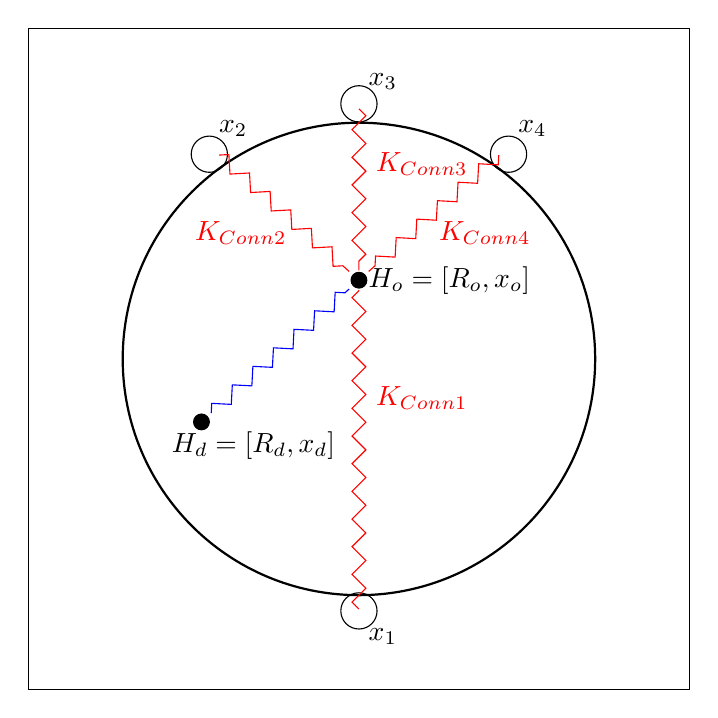
\begin{tikzpicture}
\tikzstyle{spring}=[thick,decorate,decoration={zigzag,pre length=0.3cm,post length=0.3cm,segment length=5}]
 \draw [black] (0.8,0.8) rectangle (9.2,9.2);
  \draw [black, thick] (5,5) circle [radius=3];
 \node (x3) at (5,8.3){} ;
   \node (x1)at (5,1.7){} ;
    \node (x2) at (3.1,7.7){} ;
     \node (x4) at (6.9,7.7){} ;
     \node (Ho) at (5,6){};
     \node (Hd) at (3,4.2){};
     
     \node [above right] at (5,8.3){$x_3$} ;
   \node [below right] at (5,1.7){$x_1$} ;
    \node [above right] at (3.1,7.7){$x_2$} ;
     \node [above right] at (6.9,7.7){$x_4$} ;
     \node [right]at (5,6){$H_o=[R_o,x_o]$};
     \node [below right]at (2.5,4.2){$H_d=[R_d,x_d]$};
     
     \node [red]at (5.8,4.5){$K_{Conn1}$};
     \node [red]at (3.5,6.6){$K_{Conn2}$};
     \node [red]at (5.8,7.48){$K_{Conn3}$};
     \node [red]at (6.6,6.6){$K_{Conn4}$};
     
    \draw  (5,8.24) circle [radius=0.23];
    \draw  (5,1.8) circle [radius=0.23];
     \draw  (3.1,7.6) circle [radius=0.23];
      \draw  (6.9,7.6) circle [radius=0.23];
       \draw  [fill=black] (5,6) circle [radius=0.1];
       \draw  [fill=black] (3,4.2) circle [radius=0.1];
      
      \draw[red,decorate,decoration=zigzag] (x3) -- (Ho);
      \draw[red,decorate,decoration=zigzag] (x1) -- (Ho);
      \draw[red,decorate,decoration=zigzag] (x2) -- (Ho);
      \draw[red,decorate,decoration=zigzag] (x4) -- (Ho);
       \draw[blue,decorate,decoration=zigzag] (Hd) -- (Ho);
%  \draw [gray] (6,0) arc [radius=1, start angle=45, end angle= 120]; 
%   \pszigzag[coilheight=0.5](0,0)(3.5,0)
%       \uput*[0](3.5,0){0.50}
 \end{tikzpicture}

%\begin{tikzpicture}[M1/.style={rectangle,draw=black,minimum size=2cm,thick}]
%
%    \tikzstyle{spring}=[thick,decorate,decoration={zigzag,pre length=0.3cm,post length=0.3cm,segment length=5}]
%    \tikzstyle{ground}=[fill,pattern=north east lines,draw=none,minimum width=0.75cm,minimum height=0.3cm]
%    \node [M1] (M1) {};
%    \node (wall1) [ground, minimum width=3cm,yshift=-3cm] {};
%    \draw (wall1.north west) -- (wall1.north east);
%    \draw [spring] (wall1.170) -- ($(M1.south east)!(wall1.170)!(M1.south west)$) node[pos=.5,left] {$k_2$};
%    \draw [spring] (wall1.10) -- ($(M1.south west)!(wall1.10)!(M1.south east)$) node[pos=.5,right] {$k_3$};
%    \node (wall2) [ground, minimum width=3cm,yshift=3cm] {};
%    \draw (wall2.south west) -- (wall2.south east);
%    \draw [spring] (wall2.170) -- ($(M1.north east)!(wall2.170)!(M1.north west)$) node[pos=.5,left] {$k_1$};
%    \draw [-latex,thick] (1.5,0) -- (1.5,1) node [pos=.5,right] {$x$};
%    \filldraw circle (.05) node [pos=.5,below] {\tiny $CG$};
%    \node [rotate=90,above] at (M1.west) {Mass,$m$};
%    \node at (0,-3.5) {(a)};
%        \begin{scope}[xshift=5cm]
%            \node [M1] (M1) {};
%            \node (wall1) [ground, minimum width=3cm,yshift=-3cm] {};
%            \draw (wall1.north west) -- (wall1.north east);
%            \draw [spring] (wall1) -- ($(M1.south east)!(wall1)!(M1.south west)$) node[pos=.5,left] {$k_2^*$};
%            \node (wall2) [ground, minimum width=3cm,yshift=3cm] {};
%            \draw (wall2.south west) -- (wall2.south east);
%            \draw [spring] (wall2) -- ($(M1.north east)!(wall2)!(M1.north west)$) node[pos=.5,left] {$k_1$};
%            \draw [-latex,thick] (1.5,0) -- (1.5,1) node [pos=.5,right] {$x$};
%            \filldraw circle (.05) node [pos=.5,below] {\tiny $CG$};
%            \node [rotate=90,above] at (M1.west) {Mass,$m$};
%            \node at (0,-3.5) {(b)};
%        \end{scope}
%\end{tikzpicture}
%
%\begin{tikzpicture}
%\node  (image) {\fbox{\includegraphics[width=0.25\textwidth]{initial_posture_croped}}};
%\end{tikzpicture}
%
%
%
%\begin{pspicture}(0,-4)(5,5)
% \pszigzag(0,4)(3.5,4) { \psset{linewidth=0.2pt}
%  \psline[arrowscale=2,tbarsize=3mm]{|<->|}(4.5,3.5)(4.5,4.5) 
%  \psline[linestyle=dashed](2.5,4.5)(4.5,4.5)
%   \psline[linestyle=dashed](2.75,3.5)(4.5,3.5)
%    \psline[arrowscale=2,tbarsize=3mm]{|<->|}(1.75,3.2)(2.75,3.2)
%     \uput[-90](2.15,3){\footnotesize\texttt{coilheight$\times$coilwidth}} } 
%    \uput*[0](3.5,4){coilwidth}
%     \pszigzag[coilheight=0.75](0,1.5)(3.6,1.5) 
%     \uput*[0](3.5,1.5){0.75}
%      \pszigzag[coilheight=0.5](0,0)(3.5,0)
%       \uput*[0](3.5,0){0.50}
%        \pszigzag[coilheight=1.25](0,-1.5)(3.5,-1.5) 
%        \uput*[0](3.5,-1.5){1.25} 
%        \pszigzag*[coilheight=0.5](0,-3)(3.5,-3) 
%        \uput*[0](3.5,-3){0.50}
%\end{pspicture}
%\end{document}